% Rebuild with latex -interaction=nonstopmode -halt-on-error plug-tiles.tex
% then dvisvgm --no-fonts --exact --bbox=papersize plug-tiles.dvi -o plug-tiles.svg.
\documentclass[tikz,border=5pt]{standalone}
\newcommand{\tile}[3]{%
  \begin{scope}[shift={(#2,#3)}]
    \draw[line width=0.9pt] (0,0) rectangle (1,1);
    \node[left=4pt] at (0,0.5) {#1};
  \end{scope}%
}
\begin{document}
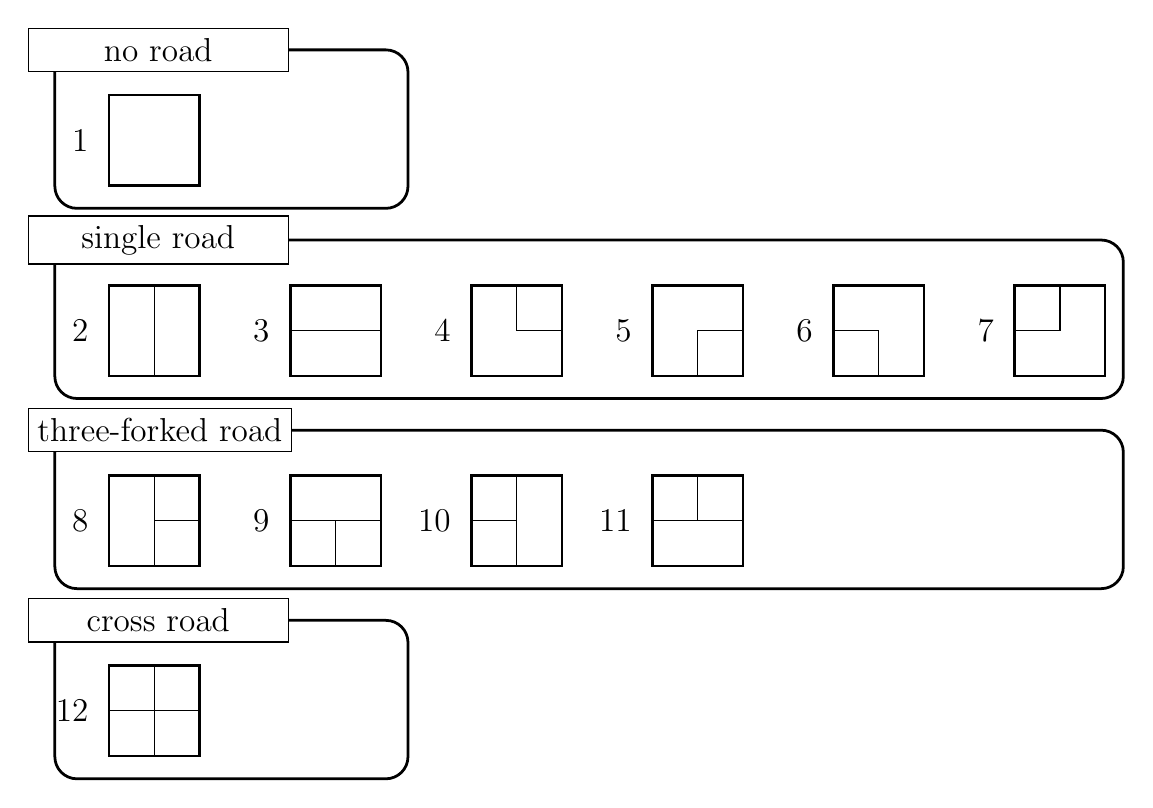
\begin{tikzpicture}[x=1.15cm,y=1.15cm,font=\large]
  % Every road reaches a tile edge at its midpoint.
  \draw[rounded corners=8pt,line width=1pt] (-0.6,4.8) rectangle (3.3,6.55);
  \draw[rounded corners=8pt,line width=1pt] (-0.6,2.7) rectangle (11.2,4.45);
  \draw[rounded corners=8pt,line width=1pt] (-0.6,0.6) rectangle (11.2,2.35);
  \draw[rounded corners=8pt,line width=1pt] (-0.6,-1.5) rectangle (3.3,0.25);
  \foreach \y/\label in {6.55/{no road},4.45/{single road},2.35/{three-forked road},0.25/{cross road}} {
    \node[draw,fill=white,anchor=west,minimum width=3.3cm,minimum height=0.55cm]
      at (-0.9,\y) {\label};
  }
  % 1: empty tile.
  \draw[line width=0.9pt] (0,5.05) rectangle (1,6.05);
  \node[left=4pt] at (0,5.55) {1};
  % 2--7: the two straight tiles and the four right-angle tiles.
  \tile{2}{0}{2.95}
  \draw (0.5,3.95) -- (0.5,2.95);
  \tile{3}{2}{2.95}
  \draw (2,3.45) -- (3,3.45);
  \tile{4}{4}{2.95}
  \draw (4.5,3.95) -- (4.5,3.45) -- (5,3.45);
  \tile{5}{6}{2.95}
  \draw (7,3.45) -- (6.5,3.45) -- (6.5,2.95);
  \tile{6}{8}{2.95}
  \draw (8,3.45) -- (8.5,3.45) -- (8.5,2.95);
  \tile{7}{10}{2.95}
  \draw (10.5,3.95) -- (10.5,3.45) -- (10,3.45);
  % 8--11: T junctions, with the missing edge rotating clockwise.
  \tile{8}{0}{0.85}
  \draw (0.5,1.85) -- (0.5,0.85) (0.5,1.35) -- (1,1.35);
  \tile{9}{2}{0.85}
  \draw (2,1.35) -- (3,1.35) (2.5,1.35) -- (2.5,0.85);
  \tile{10}{4}{0.85}
  \draw (4.5,1.85) -- (4.5,0.85) (4,1.35) -- (4.5,1.35);
  \tile{11}{6}{0.85}
  \draw (6,1.35) -- (7,1.35) (6.5,1.35) -- (6.5,1.85);
  % 12: the four-way junction.
  \tile{12}{0}{-1.25}
  \draw (0.5,-0.25) -- (0.5,-1.25) (0,-0.75) -- (1,-0.75);
\end{tikzpicture}
\end{document}
